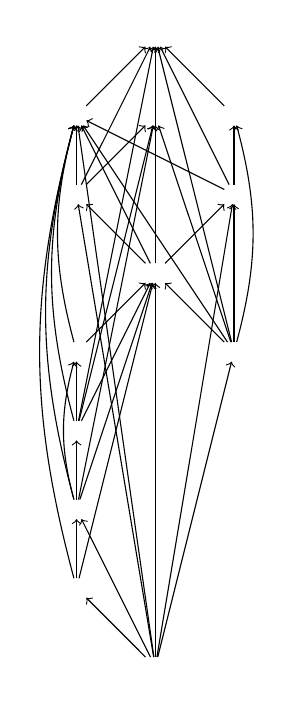
\begin{tikzpicture}

  \node (00)              {};
  \node (01) [right of=00] {\rktdot};
  \node (02) [right of=01] {};
       
  \node (10) [below of=00] {\rktdot};
  \node (11) [below of=01] {\rktdot};
  \node (12) [below of=02] {\rktdot};

  \node (20) [below of=10] {\rktdot};
  \node (21) [below of=11] {};
  \node (22) [below of=12] {\rktdot};

  \node (30) [below of=20] {};
  \node (31) [below of=21] {\rktdot};
  \node (32) [below of=22] {};

  \node (40) [below of=30] {\rktdot};
  \node (41) [below of=31] {};
  \node (42) [below of=32] {\rktdot};

  \node (50) [below of=40] {\rktdot};
  \node (51) [below of=41] {};
  \node (52) [below of=42] {};

  \node (60) [below of=50] {\rktdot};
  \node (61) [below of=51] {};
  \node (62) [below of=52] {};

  \node (70) [below of=60] {\rktdot};
  \node (71) [below of=61] {};
  \node (72) [below of=62] {};

  \node (81) [below of=71] {\rktdot};

  %% -- edges
  %% gregor-structs
  \draw[->] (10) -- (01);
  %% hmsn
  \draw[->] (11) -- (01);
  %% ymd
  \draw[->] (12) -- (01);
  %% date
  \draw[->] (22) -- (10);
  \draw[->] (22) -- (01);
  \draw[->] (22) -- (12);
  %% time
  \draw[->] (20) -- (01);
  \draw[->] (20) -- (10);
  \draw[->] (20) -- (11);
  %% datetime
  \draw[->] (31) -- (20);
  \draw[->] (31) -- (22);
  \draw[->] (31) -- (11);
  \draw[->] (31) -- (10);
  \draw[->] (31) -- (01);
  %% diff
  \draw[->] (42) -- (01);
  \draw[->] (42) -- (10);
  \draw[->] (42) -- (11);
  \draw[->] (42) edge[bend right=15] (12);
  \draw[->] (42) -- (22);
  \draw[->] (42) -- (31);
  %% moment-base
  \draw[->] (40) edge[bend left=15] (10);
  \draw[->] (40) -- (31);
  %% offset-resolvers
  \draw[->] (50) -- (01);
  \draw[->] (50) edge[bend left=15] (10);
  \draw[->] (50) -- (11);
  \draw[->] (50) -- (31);
  \draw[->] (50) -- (40);
  %% moment
  \draw[->] (60) edge[bend left=15] (10);
  \draw[->] (60) -- (11);
  \draw[->] (60) -- (31);
  \draw[->] (60) edge[bend left=15] (40);
  \draw[->] (60) -- (50);
  %% clock
  \draw[->] (70) edge[bend left=15] (10);
  \draw[->] (70) -- (31);
  \draw[->] (70) -- (60);
  %% main
  \draw[->] (81) -- (10);
  \draw[->] (81) -- (20);
  \draw[->] (81) -- (22);
  \draw[->] (81) -- (31);
  \draw[->] (81) -- (60);
  \draw[->] (81) -- (70);
  \draw[->] (81) -- (42);

\end{tikzpicture}
